\documentclass[10pt,
  aspectratio=169,
  serif,
  mathserif,
  professionalfont,
  compress,
  handout,
  % table,
  % svgnames
  ]{beamer}\usepackage[]{graphicx}\usepackage[]{color}
% maxwidth is the original width if it is less than linewidth
% otherwise use linewidth (to make sure the graphics do not exceed the margin)
\makeatletter
\def\maxwidth{ %
  \ifdim\Gin@nat@width>\linewidth
    \linewidth
  \else
    \Gin@nat@width
  \fi
}
\makeatother

\definecolor{fgcolor}{rgb}{1, 1, 0.941}
\newcommand{\hlnum}[1]{\textcolor[rgb]{0.804,0.718,0.71}{#1}}%
\newcommand{\hlstr}[1]{\textcolor[rgb]{0.604,0.753,0.804}{#1}}%
\newcommand{\hlcom}[1]{\textcolor[rgb]{0.439,0.502,0.565}{#1}}%
\newcommand{\hlopt}[1]{\textcolor[rgb]{1,1,0.941}{#1}}%
\newcommand{\hlstd}[1]{\textcolor[rgb]{1,1,0.941}{#1}}%
\newcommand{\hlkwa}[1]{\textcolor[rgb]{0.941,0.902,0.549}{#1}}%
\newcommand{\hlkwb}[1]{\textcolor[rgb]{1,0.871,0.678}{#1}}%
\newcommand{\hlkwc}[1]{\textcolor[rgb]{0.545,0.941,0.702}{#1}}%
\newcommand{\hlkwd}[1]{\textcolor[rgb]{0.545,0.941,0.902}{#1}}%
\let\hlipl\hlkwb

\usepackage{framed}
\makeatletter
\newenvironment{kframe}{%
 \def\at@end@of@kframe{}%
 \ifinner\ifhmode%
  \def\at@end@of@kframe{\end{minipage}}%
  \begin{minipage}{\columnwidth}%
 \fi\fi%
 \def\FrameCommand##1{\hskip\@totalleftmargin \hskip-\fboxsep
 \colorbox{shadecolor}{##1}\hskip-\fboxsep
     % There is no \\@totalrightmargin, so:
     \hskip-\linewidth \hskip-\@totalleftmargin \hskip\columnwidth}%
 \MakeFramed {\advance\hsize-\width
   \@totalleftmargin\z@ \linewidth\hsize
   \@setminipage}}%
 {\par\unskip\endMakeFramed%
 \at@end@of@kframe}
\makeatother

\definecolor{shadecolor}{rgb}{.97, .97, .97}
\definecolor{messagecolor}{rgb}{0, 0, 0}
\definecolor{warningcolor}{rgb}{1, 0, 1}
\definecolor{errorcolor}{rgb}{1, 0, 0}
\newenvironment{knitrout}{}{} % an empty environment to be redefined in TeX

\usepackage{alltt}

% Tamanho de fonte e distância entre linhas.
\renewenvironment{knitrout}{
  \renewcommand{\baselinestretch}{0.75}%\tiny
}{}

%-----------------------------------------------------------------------
% Pacotes padrões.

% Fontes.
\usepackage{palatino}
\usepackage{eulervm}
\usepackage{inconsolata}

% Esses pacotes dão clash.
% http://tex.stackexchange.com/questions/51488/option-clash-with-xcolor-and-tikz
% \usepackage{xcolor} %% opções no \documentclass{} para evitar clash.
% \definecolor{mycolor}{rgb}{0.13,0.53,0.53}
% \definecolor{mycolor2}{rgb}{0.725,0,0.18}

\usepackage{hyperref}
 \hypersetup{colorlinks, allcolors=., urlcolor=structure}
% \hypersetup{colorlinks}

\usepackage[brazil]{babel}
\usepackage[utf8]{inputenc}
\usepackage{graphicx}
\usepackage{amsmath, amsfonts, amssymb, amsxtra, amsthm, icomma}
\usepackage{geometry, calc, setspace, indentfirst}
% \usepackage{colortbl}
\usepackage{enumerate}
\usepackage{float}

\usepackage{subfigure}

\usepackage[hang]{caption}
\captionsetup{font=footnotesize,
  labelfont=footnotesize,
  labelsep=period}

% Listas em duas colulas.
\usepackage{multicol}
\newenvironment{itemize2}{%
  \vspace*{-1em}
  \begin{itemize}
    \begin{multicols}{2}
    }{%
    \end{multicols}
  \end{itemize}
}

% Texto no corpo do beamer justificado.
\usepackage{ragged2e}
\justifying

%-----------------------------------------------------------------------

% A lot of options:
% http://latex-community.org/forum/viewtopic.php?f=55&t=17646
\useoutertheme[
  width=60pt,
  height=30pt,
  right,
  hideothersubsections
  ]{sidebar}

\makeatletter
\setbeamertemplate{caption}[numbered]
\setbeamertemplate{section in toc}[sections numbered]
\setbeamertemplate{subsection in toc}[subsections numbered]
\setbeamertemplate{sections/subsections in toc}[ball]{}
\setbeamertemplate{section in sidebar right}[sections numbered]
\setbeamertemplate{frametitle continuation}{\gdef\beamer@frametitle{}}
\setbeamertemplate{navigation symbols}{} %% Retira a barra de navegação.
% \setbeamertemplate{blocks}[rounded][shadow=FALSE]
% \setbeamercolor{block title}{fg=structure, bg=mycolor!20!white}
\makeatother

% Frames com sessão e/ou subsessão.
\addtobeamertemplate{frametitle}{
  \let\insertframetitle\insertsubsectionhead}{}
\makeatletter
\CheckCommand*\beamer@checkframetitle{
  \@ifnextchar\bgroup\beamer@inlineframetitle{}}
\renewcommand*\beamer@checkframetitle{
  \global\let\beamer@frametitle\relax\@ifnextchar\bgroup
  \beamer@inlineframetitle{}}
\makeatother

%-----------------------------------------------------------------------
% Comandos.

\newcommand{\n}[1]{\textbf{#1}}

%-----------------------------------------------------------------------

\AtBeginSection[]{
  \begin{frame}[c,allowframebreaks]
    \begin{center}
      {\thesection} \\ \vspace{0.3cm}
      \parbox{0.6\textwidth}{
        \centering {\Large \textcolor{structure}{\insertsection}}}\\
    \end{center}
  \end{frame}
}

%-----------------------------------------------------------------------
% Definições dos proprietários.

\title[TH MCGLM]{
  \LARGE Testes de hipótese em Modelos\\  Multivariados de Covariância  \\ Linear Generalizada (McGLM)}


\subtitle{Uma visão geral}


\author[Lineu Alberto]{%\small
  Lineu Alberto Cavazani de Freitas \\
  \texttt{lineuacf@gmail.com}
}

\institute[UFPR]{
  PPG Informática \\
  Data Science \& Big Data \\
  Universidade Federal do Paraná\\

  \vspace{1em}
  \href{}{https://lineu96.github.io/st/}
}
\date{}

\logo{
\includegraphics[width=1.5cm]{img/dsbd1x4-rect.png}} 

\usebackgroundtemplate{
  
\includegraphics[width=\paperwidth]{img/ufpr-fundo.jpg}
}

%=======================================================================
%=======================================================================
\IfFileExists{upquote.sty}{\usepackage{upquote}}{}
\begin{document}

\frame{
  \titlepage
}

% Tabela de conteúdo no início dos slides.
% \begin{frame}{Conteúdo}
%   \small{\tableofcontents}
% \end{frame}

%-----------------------------------------------------------------------



% -----------------------------------------------------------------

\section{Quem sou eu}

\begin{frame}
\frametitle{explanation}
\begin{columns}
\begin{column}{0.7\textwidth}
   
   \textbf{Quem sou eu}
   
   \begin{itemize}

  \item Estatístico formado pela \href{https://www.ufpr.br/portalufpr/}{Universidade Federal do Paraná (UFPR)} em 2019.

  \item Atividades participadas na graduação:
    \begin{itemize}
      \item Programa de Educação Tutorial (\href{https://pet.leg.ufpr.br/}{PET-Estatística UFPR}).
      \item Monitoria da disciplina de \href{https://lineu96.github.io/glm/}{Modelos Lineares Generalizados (CE225)} na UFPR.
      \item Estágio no Núcleo de Estatística e Monitoramento da CGJ (\href{https://www.tjpr.jus.br/corregedoria?p_p_id=101_INSTANCE_hBdlYcS1yEFH&p_p_lifecycle=0&p_p_state=normal&p_p_mode=view&p_p_col_id=column-1&p_p_col_count=1&a_page_anchor=17290920}{NEMOC-TJPR}).
      \item Estágio no \href{https://banco.bradesco/html/classic/promocoes/hub-credito/index.shtm}{Departamento de Inteligência de Crédito do Banco Bradesco S.A}.
    \end{itemize}
  
  \end{itemize}
\end{column}
\begin{column}{0.3\textwidth}  %%<--- here
    \begin{center}
     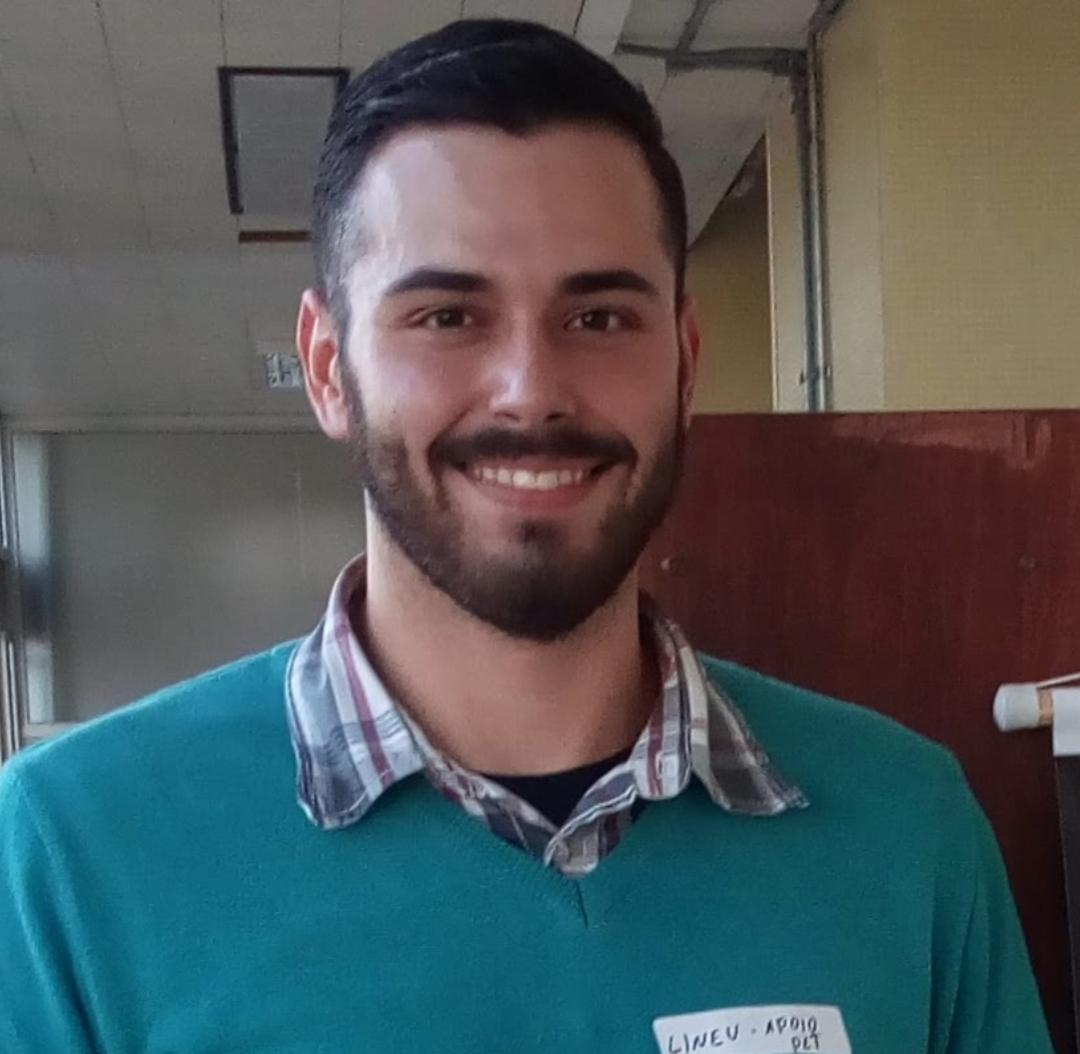
\includegraphics[width=\textwidth]{img/eu3.jpeg}
     \end{center}
\end{column}
\end{columns}
\end{frame}

\begin{frame}[c, allowframebreaks]

\begin{center}  
    \includegraphics[width=10cm]{img/col1.png}  
  \end{center}

\end{frame}

\begin{frame}[c, allowframebreaks]

\begin{center}  
    \includegraphics[width=10cm]{img/col2.png}  
  \end{center}

\end{frame}

\begin{frame}[c, allowframebreaks]

  \textbf{Onde estou hoje}

  \begin{itemize}

  \item Atualmente mestrando no \href{http://www.prppg.ufpr.br/ppginformatica/?lang=pb}{Programa de Pós Graduação em Informática da UFPR} sob a orientação dos professores:
  
  \begin{itemize}
    \item \href{http://www.leg.ufpr.br/~wagner/}{Wagner Hugo Bonat}.
    \item \href{https://web.inf.ufpr.br/mazalves/}{Marco Antonio Zanata Alves}. 
  \end{itemize}

  \item Inserido na área de concentração Ciência da Computação, linha de pesquisa Tecnologia da Informação e grupo de pesquisa \href{https://web.inf.ufpr.br/dsbd/}{Data Science \& Big Data}.
  
  \end{itemize}

\end{frame}

% -----------------------------------------------------------------

\section{Um pouco sobre o PPGINF}

\begin{frame}[c, allowframebreaks]
  
  \begin{center}  
    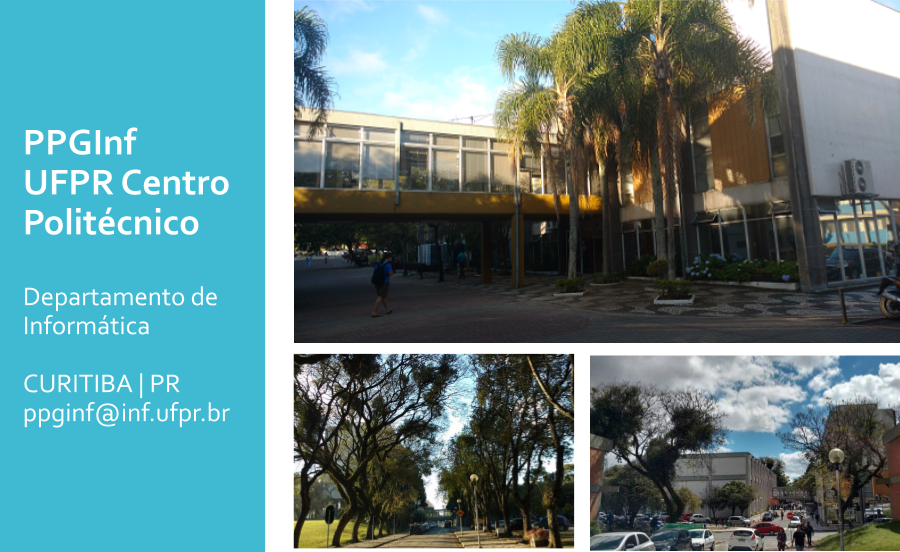
\includegraphics[width=11.5cm]{img/ppginf.png}  
  \end{center}

\end{frame}

\begin{frame}[c, allowframebreaks]
  
  \textbf{Visão geral}
  
  \begin{itemize}

  \item O Programa é oferecido pelo \href{https://web.inf.ufpr.br/dinf/}{Departamento de Informática da UFPR}. 

  \item Tem conceito 5 de 7 possíveis atribuídos na última avaliação pela \href{https://www.gov.br/capes/pt-br}{CAPES} (5 equivale a "muito bom" na escala).
  
  \item Oferece mestrado desde 1996.
  
  \item Oferece doutorado desde 2009.
  
  \end{itemize}

\end{frame}

\begin{frame}[c, allowframebreaks]
  
  \textbf{Áreas, linhas e grupos de pesquisa}
  
  \begin{itemize}

  \item No programa a área de concentração é Ciência da Computação.

  \item Existem 3 linhas de pesquisa:
  \begin{itemize}
    \item \href{http://www.prppg.ufpr.br/ppginformatica/index.php/inteligencia-computacional/?lang=pb}{Inteligência computacional}.
    \item \href{http://www.prppg.ufpr.br/ppginformatica/index.php/redes-e-sistemas-distribuidos/?lang=pb}{Redes e sistemas distribuídos}.
    \item \href{http://www.prppg.ufpr.br/ppginformatica/index.php/tecnologia-da-informacao/?lang=pb}{Tecnologia da Informação}.
  \end{itemize}
  
  \item Cada uma das linhas possuem diversos grupos de pesquisa.
  
  \end{itemize}

\end{frame}

\begin{frame}[c, allowframebreaks]
  
  \textbf{Grupos de pesquisa}
  
  \begin{table}[]
\begin{tabular}{cl}
\hline
\multicolumn{2}{c}{Inteligência Computacional}                                             \\ \hline
\multicolumn{1}{l}{} 
                     &                                                                     \\
C-Bio                & Computação Bioinspirada, Meta-heurísticas e Aprendizagem de Máquina \\
\multicolumn{1}{l}{} &                                                                     \\
IMAGO                & Visão Computacional, Computação Gráfica e Processamento de Imagens  \\
\multicolumn{1}{l}{} &                                                                     \\
LIAMF                & Inteligência Artificial e Métodos Formais                           \\
\multicolumn{1}{l}{} &                                                                     \\
LIC                  & Sistemas Tutores Inteligentes                                       \\
\multicolumn{1}{l}{} &                                                                     \\
TEORIA               & Teoria da Computação, Otimização e Combinatória                     \\
\multicolumn{1}{l}{} &                                                                     \\
VRI                  & Visão, Robótica e Imagem                                            \\
                     &                                                                     \\ \hline
\end{tabular}
\label{tab:my-table}
\end{table}

\end{frame}

\begin{frame}[c, allowframebreaks]
  
  \textbf{Grupos de pesquisa}
  
\begin{table}[]
\begin{tabular}{cl}
\hline
\multicolumn{2}{c}{Redes e Sistemas Distribuídos}                                                                                                                              \\ \hline
                     &                                                                     \\
CCSC   & Centro de Ciência de Segurança Computacional                                                                                                                          \\
       &                                                                                                                                                                       \\
LARSIS & Laboratório de Redes, Sistemas Distribuídos e Segurança                                                                                                               \\
       &                                                                                                                                                                       \\
NR2    & \begin{tabular}[c]{@{}l@{}}Gerenciamento de Redes de Computadores, Sistemas Distribuídos, \\ Redes Sem Fio, Segurança, Modelagem e Análise de Desempenho\end{tabular} \\
       &                                                                                                                                                                       \\
LSE    & Laboratório de Sistemas Embarcados                                                                                                                                    \\
       &                                                                                                                                                                       \\
HiPES  & \begin{tabular}[c]{@{}l@{}}High Performance and Efficient Systems. (Computer Architecture, \\ Security and Networks)\end{tabular}                                     \\ 
                     &                                                                     \\\hline
\end{tabular}
\label{tab:my-table}
\end{table}

\end{frame}

\begin{frame}[c, allowframebreaks]
  
  \textbf{Grupos de pesquisa}
  
\begin{table}[]
\begin{tabular}{cl}
\hline
\multicolumn{2}{c}{Tecnologia da Informação}              \\ \hline
                     &                                                                     \\
BD   & Banco de Dados                                     \\
     &                                                    \\
BDGE & Banco de Dados de Grande Escala                    \\
     &                                                    \\
FAES & Fundamentos e Aplicações em Engenharia de Software \\
     &                                                    \\
C3SL & Centro de Computação Científica e Software Livre   \\
     &                                                    \\
GrES & Engenharia de Software                             \\
     &                                                    \\
IHC  & Interação Humano-Computador                        \\
     &                                                    \\
DSBD & Data Science and Big Data                          \\ 
                     &                                                                     \\
                     \hline
\end{tabular}
\label{tab:my-table}
\end{table}

\end{frame}

\begin{frame}[c, allowframebreaks]

\textbf{Por que é um programa interessante para nós estatísticos?}

  \begin{itemize}

  \item Porque é interessante se arriscar em outra área.

  \item Pela variedade de grupos de pesquisa.
  
  \item Pela flexibilidade do currículo:
  
  \begin{itemize}
    \item 2 disciplinas obrigatórias.
    \item 3 disciplinas optativas.
    \item Prática em docência (para bolsistas).
    
  \end{itemize}
  
  \item Pelo \href{https://web.inf.ufpr.br/dsbd/}{DSBD}.
  
  \end{itemize}

\end{frame}

\begin{frame}[c, allowframebreaks]

\textbf{O DSBD}

  \begin{itemize}

  \item \href{https://web.inf.ufpr.br/dsbd/}{Laboratório de Data Science \& Big Data}.

  \item Criado em 2018 em uma parceria entre os departamentos de Informática (\href{https://web.inf.ufpr.br/dinf/}{DINF}) e Estatística (\href{http://www.est.ufpr.br/}{DEST}).
  
  \item É uma possibilidade para quem quer seguir na academia, em Curitiba, seguindo trabalhando de alguma forma com métodos estatísticos (ou não), sem perder o contato com o (\href{http://www.est.ufpr.br/}{DEST}). 
  
  \item É uma oportunidade para levar nossos conhecimentos adquiridos no bacharelado em Estatística e combiná-los com conhecimentos a serem adquiridos na Ciência da Computação.
  
  \end{itemize}

\begin{center}  
  
\includegraphics[width=6cm]{img/dsbd1x4.png}  
\end{center}

\end{frame}

% -----------------------------------------------------------------

\section{Minha pesquisa}

\begin{frame}[c, allowframebreaks]
  
  \textbf{Onde tudo começou}
  
  \begin{itemize}

  \item O projeto teve início em 2018 quando eu e uma colega de curso (\href{https://br.linkedin.com/in/jhecaetano}{Jhenifer Caetano Veloso}), desenvolvemos nosso TCC sob orientação do professor Wagner. 

  \item O título do trabalho foi "\href{https://lineu96.github.io/st/projects/manova/}{Análise de Variância Multivariada para Dados Não Gaussianos via Teste Wald}".
  
  \end{itemize}

\end{frame}

\begin{frame}[c, allowframebreaks]

\begin{center}  
  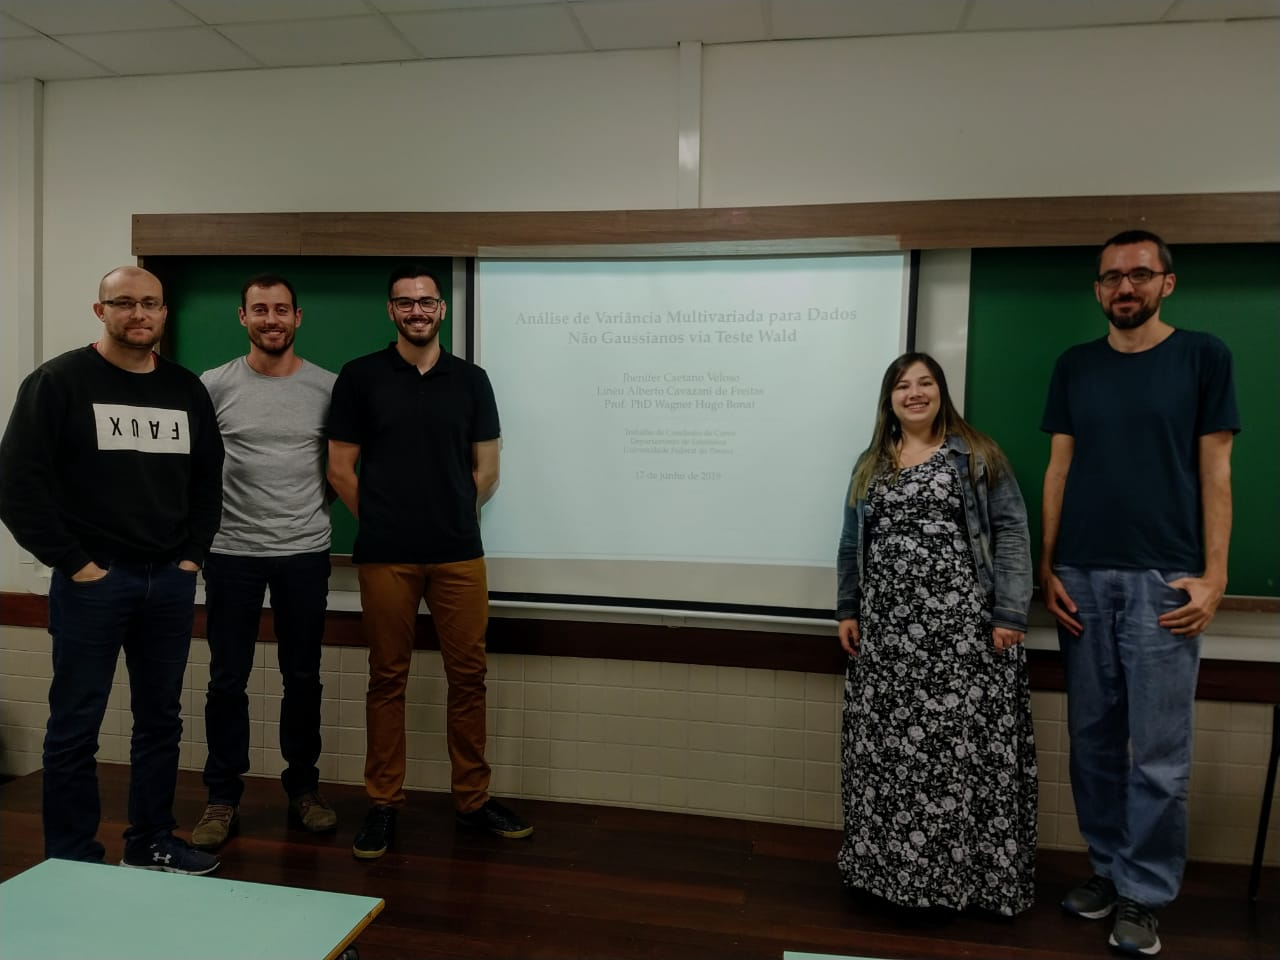
\includegraphics[width=9.4cm]{img/tcc.jpg}  
\end{center}

\end{frame}

\begin{frame}[c, allowframebreaks]
  
  \textbf{Plano para o mestrado}
  
  \begin{itemize}
  
  \item A ideia da minha pesquisa de mestrado é dar continuidade e ampliar o foco do trabalho que teve início na graduação.
  
  \item O título atual do trabalho é "Testes de hipótese em Modelos Multivariados de Covariância Linear Generalizada (McGLM)".

  \end{itemize}

\end{frame}

\begin{frame}[c, allowframebreaks]
  
  \textbf{Nosso objetivo é:}
  
  \begin{itemize}
    \item Adaptar o teste Wald para realização de testes de hipótese gerais sobre parâmetros de Modelos Multivariados de Covariância Linear Generalizada (McGLM).
    
    \item Implementar funções para efetuar tais testes, bem como funções para efetuar Análises de Variância e Análises de Variância Multivariadas para os McGLM.
    
    \item Demonstrar as propriedades e comportamento dos testes propostos com base em estudos de simulação.
    
    \item Demonstrar o potencial de aplicação das metodologias discutidas com base na aplicação a conjuntos de dados reais.
    
  \end{itemize}

\end{frame}



\begin{frame}[c, allowframebreaks]
  
  \textbf{Plano de hoje}
  
  \begin{itemize}

  \item Devido ao público alvo da palestra vamos tentar falar pouco de teoria (especificações, fórmulas, etc) e mais sobre ideias (pra que as coisas servem e porque utilizá-las é interessante).
  
  \item Vamos tentar construir uma linha de raciocínio falando desde o básico até chegar na classe de modelos que eu trabalho pra poder falar sobre o que estamos desenvolvendo.
  
  \end{itemize}

\end{frame}

\begin{frame}[c, allowframebreaks]
  
  \textbf{Vamos conversar sobre:}
  
  \begin{itemize}

  \item Quais as etapas do processo de análise de um conjunto de dados.
  
  \item Modelos de regressão de uma forma bastante didática (para que servem, quais os tipos, pressupostos gerais).
  
  \item McGLM que é classe de modelos de regressão sobre a qual trabalhamos.
  
  \item Como podemos aplicar teste de hipótese sobre os parâmetros do modelo desta classe.
  
  \end{itemize}

\end{frame}

% -----------------------------------------------------------------

\section{Etapas do processo de análise}

\begin{frame}[c, allowframebreaks]

\textbf{O processo de análise consiste em:}

  \begin{itemize}

  \item Definição do problema.

  \item Planejamento do estudo.

  \item Coleta de dados.

  \item Análise dos dados:
    \begin{itemize}
      \item Análise exploratória.
      \item Aplicação de métodos mais sofisticados que permitam generalizar os resultados para a população.
    \end{itemize}

  \item Interpretação dos resultados.
  
  \end{itemize}

\end{frame}

% -----------------------------------------------------------------

\section{Conjunto de dados}

\begin{frame}[c, allowframebreaks]

\begin{itemize}
  \item Um conjunto de dados ou "dataset" é uma coleção de dados normalmente tabulados em que organiza-se elementos ou indivíduos e suas características (variáveis). 

  \item Uma forma conveniente de se organizar os dados é da seguinte forma:
    \begin{itemize}
      \item Cada coluna representa uma variável.
      \item Cada linha representa uma observação.
      \item Cada célula representa o valor observado no elemento $i$ na variável $j$.
    \end{itemize}
\end{itemize}

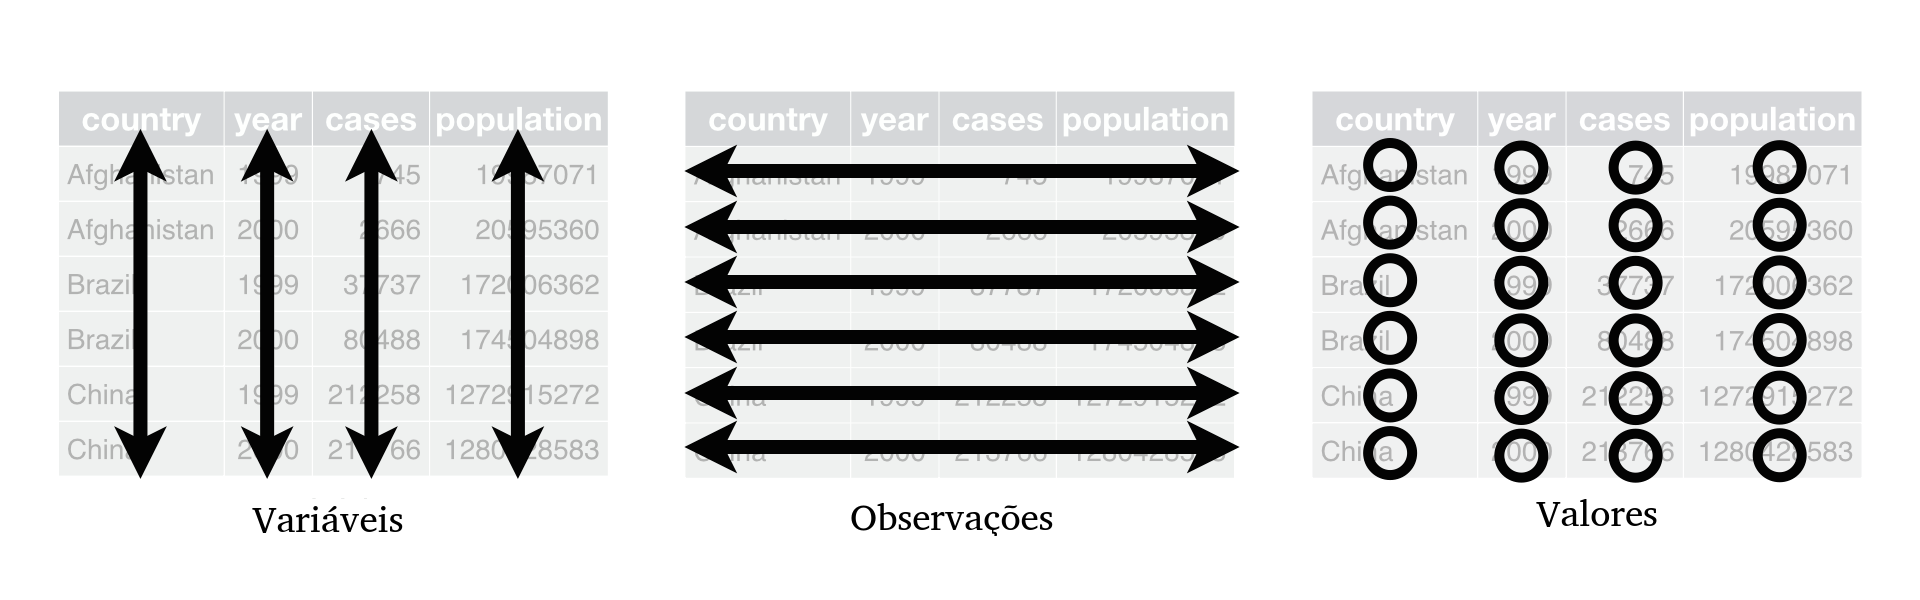
\includegraphics[width=\textwidth]{img/tidy-data_t.png}

\end{frame}

% -----------------------------------------------------------------

\section{Modelos de Regressão}

\begin{frame}[c, allowframebreaks]

\begin{itemize}
  \item Nos casos univariados, estes modelos associam uma única variável resposta, a uma ou mais variáveis explicativas.

  \item De forma geral, um modelo de regressão é uma expressão matemática que relaciona a média da variável resposta às variáveis preditoras (covariáveis).
  
  \item A grosso modo, estimamos parâmetros que medem a força de associação da variável explicativa sobre a variável resposta.
  
  \item A variável resposta segue uma distribuição de probabilidade condicional às covariáveis e a média é descrita por um preditor linear.
\end{itemize}

\end{frame}

\begin{frame}[c, allowframebreaks]

\begin{itemize}
  \item Há casos em que são coletadas mais de uma resposta por unidade experimental.
  
  \item E há o interesse de modelá-las em função de um conjunto de variáveis explicativas.
  
  \item Saímos então do cenário univariado (apenas uma resposta) e passamos para o multivariado (mais de uma resposta).
  
  \item Existem classes de modelos univariados e multivariados.
  
\end{itemize}

\end{frame}

\begin{frame}[c, allowframebreaks]

São uma das principais e mais difundidas ferramentas utilizadas em diversas áreas do conhecimento, sendo comum o interesse em:

\begin{itemize}
  \item Explicar a associação entre uma ou mais variáveis resposta e um conjunto de variáveis explicativas.
  
  \item Utilizar o modelo para realizar predições para uma população.
\end{itemize}

\end{frame}

\begin{frame}[c, allowframebreaks]

\textbf{Por exemplo...}

\begin{itemize}

  \item Considere o exemplo disponível na secão 4.3.6 do livro \href{https://www.ime.usp.br/~giapaula/texto_2013.pdf}{Modelos de Regressão com Apoio Computacional} do professor \href{https://www.ime.usp.br/~giapaula/}{Gilberto A. Paula}:

  \item Os dados referem-se a um estudo sobre demanda de TV's a cabo em 40 regiões dos Estados Unidos. 

\end{itemize}

\end{frame}

\begin{frame}[c, allowframebreaks]

\textbf{Foram coletadas as variáveis como:}

\begin{itemize}

  \item Número de assinantes de TV a cabo.

  \item Número de domicílios.

  \item Percentual de domicílios com TV a cabo.

  \item Renda per capita por domicílio com TV a cabo (em USD).

  \item Dentre outras.

\end{itemize}

\textbf{O objetivo do estudo é verificar se existe associação entre o número de assinantes e as demais variáveis.}

\end{frame}

\begin{frame}[c, allowframebreaks]

\textbf{E agora?}

\begin{itemize}

  \item É um problema que faz sentido ser analisado com um modelo de regressão?

  \item Qual a variável resposta?

  \item Quais as variáveis explicativas?

  \item Devo usar um modelo univariado ou multivariado?

  \item Qual a natureza da minha variável resposta?
  
  \item Que distribuição de probabilidade devo usar para modelar o problema?
  
  \item Seria um modelo focado em explicação ou predição?

\end{itemize}

\end{frame}

\begin{frame}[c, allowframebreaks]

\textbf{Tendo essas informações somos capazes de selecionar a classe de modelos de regressão que mais se adequa ao problema que temos em mãos. E passar por etapas como:}

\begin{itemize}

  \item Ajustar o modelo.

  \item Verificar se está bem ajustado.

  \item Em caso de mal ajuste, verificar que mudanças são possíveis na especificação.

  \item Em caso de ajuste satisfatório, podemos estudar os parâmetros:
  
  \begin{itemize}
    
    \item Lembre-se, os parâmetros são quantidades que associam as variáveis explicativas com as variáveis resposta.
    
    \item Podemos formular hipóteses para verificar se estes parâmetros são iguais a determinados valores de interesse, como 0, por exemplo.
    
  \end{itemize}

\end{itemize}

\end{frame}

\begin{frame}[c, allowframebreaks]

\textbf{Existem inúmeras classes de modelos de regressão, algumas delas são:}

\begin{itemize}
 \item Modelo Linear Normal.
 \item Modelos Lineares Generalizados (GLM).
 \item Modelos de regressão local.
 \item Modelos de regressão de splines.
 \item Modelos aditivos generalizados (GAM).
 \item Modelos de efeitos aleatórios.
 \item Modelos Aditivos Generalizados para Locação, Escala e Forma (GAMLSS).
 \item Modelos de regressão multivariados.
 \item Modelos Multivariados de Covariância Linear Generalizada (McGLM).
\end{itemize}

\end{frame}

\begin{frame}[c, allowframebreaks]

\textbf{Existem inúmeras classes de modelos de regressão, algumas delas são:}

\begin{itemize}
 \item Modelo Linear Normal.
 \item Modelos Lineares Generalizados (GLM).
 \item Modelos de regressão local.
 \item Modelos de regressão de splines.
 \item Modelos aditivos generalizados (GAM).
 \item Modelos de efeitos aleatórios.
 \item Modelos Aditivos Generalizados para Locação, Escala e Forma (GAMLSS).
 \item Modelos de regressão multivariados.
 \item\textbf{ Modelos Multivariados de Covariância Linear Generalizada (McGLM).}
\end{itemize}

\end{frame}

% -----------------------------------------------------------------

\section{McGLM}

\begin{frame}[c, allowframebreaks]

\textbf{Os Modelos Lineares Generalizados (GLM)}

\begin{itemize}

  \item São uma forma de modelagem univariada para dados de diferentes naturezas, tais como dados contínuos simétricos e assimétricos, contagens, dentre outras. 
  
  \item Tais características tornam essa classe de modelos uma flexível ferramenta de modelagem aplicável a diversos tipos de problemas.

  \item Contudo, por mais flexível e discutida na literatura, essa classe apresenta duas principais restrições: 

  \begin{enumerate}
    \item A incapacidade de lidar com observações dependentes.
    \item A incapacidade de lidar com múltiplas respostas simultaneamente.
  \end{enumerate}
  
\end{itemize}

\end{frame}

\begin{frame}[c, allowframebreaks]

\textbf{Os Modelos Multivariados de Covariância Linear
Generalizada (McGLM)}

\begin{itemize}
  \item Trata-se de uma classe que contorna as duas principais restrições presentes nos GLM.
  
  \item Esta classe de modelagem comporta:

  \begin{itemize}
    \item Múltiplas respostas.
    \item Respostas de diferentes naturezas.
    \item Respostas correlacionadas.
    \item Observações não independentes.
    \item Extensões multivariadas para modelos de:
      \begin{itemize}
        \item Séries temporais.
        \item Dados longitudinais.
        \item Dados espaciais.
    \end{itemize}
  \end{itemize}
\end{itemize}

\end{frame}

% -----------------------------------------------------------------

\section{Testes de hipótese em modelos de regressão}

\begin{frame}[c, allowframebreaks]

\textbf{Qual é a importância disso?}

\begin{itemize}

  \item Como já discutimos, nos modelos de regressão estimamos parâmetros que associam variáveis explicativas às variáveis resposta.

  \item Caso tenhamos um modelo para um problema e este modelo esteja bem ajustado, podemos estudar estas estimativas a fim de melhor compreender o fenômeno estudado. 
  
  \item E extrair informações como:
  
  \begin{itemize}
    \item Quais variáveis são importantes.
    \item Quais não são.
    \item Quais delas estão positivamente ou negativamente associadas à resposta.
    \item etc.
  \end{itemize}
\end{itemize}

\end{frame}

\begin{frame}[c, allowframebreaks]

\textbf{Fazemos isto por meio de testes de hipótese.}

\hspace{1cm}

Com estes testes podemos responder perguntas como:

\begin{itemize}

  \item Existe evidência suficiente que nos permita afirmar que o parâmetro que associa determinada variável explicativa à variável resposta é igual a 0?

  \item Em outras palavras: existe evidência que nos permita afirmar que existe efeito desta variável sobre a variável resposta?

  \item Esta é a ideia dos testes de hipótese aplicados no contexto dos modelos de regressão.

\end{itemize}

\end{frame}

\begin{frame}[c, allowframebreaks]

Além de testar parâmetros individuais, podemos testar combinações de parâmetros para verificar hipóteses como: 
  
  \begin{itemize}
    
    \item Será que existe evidência suficiente que nos permita afirmar que nem a variável A nem a variável B são importantes?
    
    \item Será que ambas são importantes?
    
    \item Será que apenas uma delas é importante?
    
  \end{itemize}

\end{frame}

\begin{frame}[c, allowframebreaks]

\begin{itemize}

  \item No caso dos modelos multivariados isso se torna especialmente útil pois podemos verificar a validade de hipóteses como: 
  
  \begin{itemize}
    \item Será que determinada variável é importante em todas as resposta simultâneamente?
    
    \item Será que determinada variável é importante em ao menos uma resposta?
    
    \item Será que determinada variável não tem efeito em nenhuma das respostas?
    
  \end{itemize}

  \item Note que se trata de uma hipótese sobre múltiplos parâmetros, pois temos um valor que associa a variável para cada uma das respostas.

\end{itemize}

\end{frame}

\begin{frame}[c, allowframebreaks]

Existem alguns testes para verificar tais tipos de hipótese. Os mais famosos são:

\begin{itemize}

  \item Teste da Razão de Verossimilhanças. 
  
  \item Teste Escore.
  
  \item Teste Wald.
  
\end{itemize}

\end{frame}

\begin{frame}[c, allowframebreaks]

\textbf{Vamos retomar o exemplo...}

\hspace{1cm}

Considerando o estudo sobre demanda de TV’s a cabo em 40 regiões
dos Estados Unidos. Em que temos as seguintes variáveis:

\begin{itemize}

  \item Número de assinantes de TV a cabo.

  \item Número de domicílios.

  \item Percentual de domicílios com TV a cabo.

  \item Renda per capita por domicílio com TV a cabo (em USD).

  \item Dentre outras.

\end{itemize}

\end{frame}

\begin{frame}[c, allowframebreaks]

\begin{itemize}

  \item Digamos que agora nosso interesse seja modelar o número de assinantes de TV a cabo E o percentual de domicílios com TV a cabo.

  \item Note que temos duas variáveis resposta, ou seja, caberia utilizar uma classe de modelos multivariados (como o McGLM).

  \item Digamos que tenhamos ajustado um modelo, verificado os pressupostos, realizado uma análise de diagnóstico e que, por fim, concluímos que nosso modelo está bem ajustado.

  \item Passamos então para a etapa do estudo das estimativas dos parâmetros que associam variáveis explicativas às variáveis resposta.

\end{itemize}

\end{frame}

\begin{frame}[c, allowframebreaks]

\textbf{Vamos considerar a variável explicativa número de domicílios:}

\begin{itemize}

  \item Teríamos em mãos as estimativas de 2 parâmetros referentes ao número de domicílios:
  
  \begin{itemize}
  
    \item Um deles que associa a variável à primeira resposta.
  
    \item E outro que associa a variável à segunda resposta.
  
  \end{itemize}
  
  \item Ou seja, teremos um parâmetro que associa o número de domicílios ao número de assinantes de TV a cabo e outro que associa o número de domicílios com o percentual de domicílios com TV a cabo.
  
\end{itemize}

\end{frame}

\begin{frame}[c, allowframebreaks]
  
\begin{itemize}

  \item E então podemos efetuar testes de hipótese para verificar a questões como:
  
  \begin{itemize}
    
    \item Existe efeito do número de domicílios sobre o número de assinantes de TV a cabo? 
    
    \item Existe efeito do número de domicílios sobre o percentual de domicílios com TV a cabo?
    
    \item Existe efeito do número de domicílios sobre o número de assinantes de TV a cabo e o percentual de domicílios com TV a cabo, ambas ao mesmo tempo?
    
  \end{itemize}

\end{itemize}

\end{frame}

\section{Testes de hipótese em Modelos Multivariados de Covariância Linear Generalizada (McGLM)}

\begin{frame}[c, allowframebreaks]

\textbf{Até o momento estes testes não foram propostos para os McGLM.}

\begin{itemize}
  \item O que nós estamos fazendo no trabalho é trabalhar com o teste Wald.
  
  \item As etapas do trabalho são:
  
  \begin{itemize}
    \item Adaptar o teste para que seja aplicável no McGLM.
    
    \item Implementar funções que permitam com que usuário faça seus testes de hipótese de uma forma simples.
    
    \item Verificar, através de estudos de simulação, se o teste tem um comportamento adequado.
    
    \item Fazer aplicações a conjuntos de dados reais.
    
  \end{itemize}

\end{itemize}


\end{frame}


\begin{frame}[c, allowframebreaks]

Considerando a área de pesquisa, o trabalho teria as seguintes contribuições:

\begin{enumerate}
  \item Adaptar um teste existente para uma classe de modelos não usual mas com alto potencial de aplicação.
  \item Realizar um estudo pesado de simulação para verificar o funcionamento da forma que estamos propondo.
  \item Análisar de dados provenientes de estudos reais para demonstrar a aplicabilidade das funcionalidades.
\end{enumerate}

\end{frame}

\begin{frame}[c, allowframebreaks]

\begin{center}

  {\huge \href{https://lineu96.github.io/st/}{Obrigado!}}
  
  \vspace{0.5cm}
    
  {\normalsize \href{https://lineu96.github.io/st/}{Lineu Alberto Cavazani de Freitas}}
  
  {\normalsize \href{https://lineu96.github.io/st/}{lineuacf@gmail.com}}
  
  {\normalsize \href{https://lineu96.github.io/st/}{https://lineu96.github.io/st/}}
  
  {\normalsize \href{http://www.prppg.ufpr.br/ppginformatica/?lang=pb}{PPG Informática}}


\begin{figure} % Inicia o ambiente de figuras
  %\subfigure{ % Começa a incluir a figura fig1.pdf
  %  
\includegraphics[width=2cm]{img/logo.png}
  %} % Termina de incluir a figura fig1.pdf
  \subfigure{ % Começa a incluir a figura fig2.pdf na mesma linha da figura fig1.pdf
    
\includegraphics[width=3cm]{img/ufpr-transparent.png}
  } % Termina de incluir a figura fig2.pdf
  %\subfigure{ % Começa a incluir a figura fig3.pdf na linha abaixo
  %  
\includegraphics[width=1.4cm]{img/dsbd-2x2-trans.png}
  %} % Termina de incluir a figura fig3.pdf
\end{figure} % Fecha o ambiente de figuras

\end{center}

\end{frame}

\end{document}
